\documentclass[12pt]{article}
\newcommand{\ts}{\textsuperscript}

\usepackage[margin=1in]{geometry}
\usepackage{caption}
\usepackage{cite}
\usepackage{subcaption,graphicx}
\usepackage{lineno, blindtext}
\usepackage{float}
\usepackage{color}
\usepackage{graphicx}
\usepackage[hidelinks]{hyperref}
\usepackage{enumitem}
\usepackage{multicol}
\usepackage{fancyhdr}
\usepackage{times}
\usepackage{mathtools}
\usepackage{pdfpages}
\setlength{\parindent}{0pt}
\newcommand{\forceindent}{\leavevmode{\parindent=1em\indent}}
%\usepackage{siunitx}
\usepackage{chronology}

\usepackage[cache=false]{minted}


\title{MSE 486 Directed Study\\Report \#2 - Implementation\\ \bigskip \textbf{2 Player Texas Hold'em Poker\\Reinforcement Learning Python Bot}}
\author{Ryan Fielding - 301284210\\rafieldi@sfu.ca\\778.886.8199\\\\Supervisor: Dr. Ahmad Rad, Ph.D.\\Associate Director, School of Mechatronic Systems Engineering,\\Simon Fraser University}
\date{July $3^{rd}$, 2020}

\begin{document}

\maketitle
\newpage

{\Large \textbf{Abstract\\\\}}
This paper outlines the project progress for a directed study in machine learning, through implementation and development of an AI based bot (\textit{RLPlayer}) to learn and understand different strategies to play poker. Particularly, the game of Texas Hold'em will be the basis for this project, potentially beginning with Leduc Hold'em since it is a much simpler version of the game.\\\\
To initiate the project, the first couple weeks will be dedicated to project research, pertaining to coding language, type of machine learning to implement, project goals, requirements and more. Implementation and development will be done in Python, through the AI of reinforcement learning.\\\\
To elaborate on the overall development, first, a basic poker environment will be initialized. There is no need to develop this from scratch as there are plenty of sources to implement a gaming environment in many languages. Following, basic game playing bots will need to be setup, as well as strategic bots and honest bots. Each level of trained bot will get more and more advanced.\\\\
In parallel, to satisfy the learning outcomes of this course as well as provide a sound understanding of machine learning, research pertaining to neural networks, types and architectures of machine learning, and intensive research involving reinforcement learning will be completed. Primarily during the first few weeks of the semester. Following, an implementation period will ensue to initiate environment setup and initial machine learning implementation. Lastly, the two phases will tie together to merge research and implementation through multiple stages of training, with various parameters and according to different strategies, resulting in a well developed reinforcement learning poker playing bot.\\\\
Training these bots will mostly consist of self play and reward based learning, however other strategies will be researched, including that of DeepStack, Libratus, Pluribus and many others that are successfully based on machine learning. The reason for two player poker, instead of 3, 4 or even 6, is because with a lower number of players at play, a rule based gaming strategy is far more effective, and much easier to implement and train. As the number of players increase, the game becomes a multi-player game that requires more sophisticated strategies and potentially even player modelling.\\\\
In terms of technical specifics, Python and PyTorch will be used since it is the most user friendly language, however the core of PyTorch is written in C++, so as to preserve high speeds. In terms of computationally intensive neural network training, rather than purchase of a high quality GPU, use of CUDA to run on a Mac OS GPU, or many other hardware solutions, Google Colab. will be used since it enables the use of free GPU's for training of python neural networks for up to 12 hours \cite{colab}. Finally, training of the bot will be done through neural fictitious self-play (NFSP), and Deep Q Learning networks (DQN).

\newpage
\tableofcontents
\listoffigures
\newpage

\section{Background}
The complex game of poker requires reasoning with hidden information. When one plays a game, not only do they quantify the value of their own hand, they also aim to predict what cards the opposing players hold. Other players can even bet high when they're hand is not valuable at all, a strong tactic called \textit{bluffing}. Additionally, there are other factors that weigh in, including pot size, call size, remaining stack and more. For background information on Texas Hold'em and how it is played, see the reference \cite{tex}.\\\\
\begin{figure}[H]
    \centering
    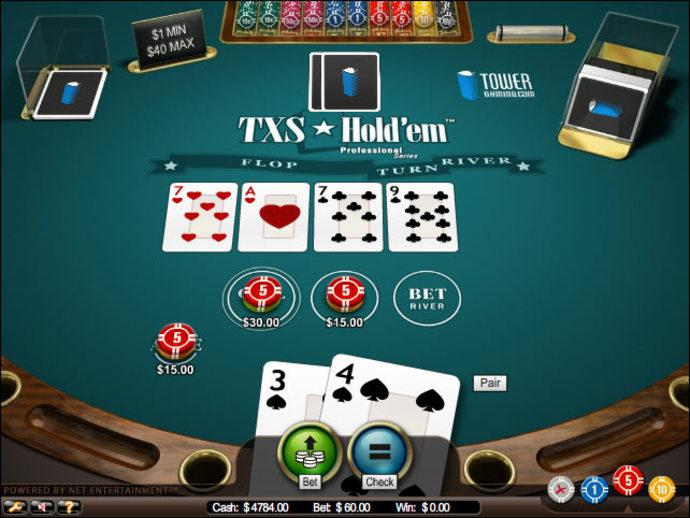
\includegraphics[width=.70\linewidth]{figures/texas.jpg}
    \caption{Online Texas Hold'em}
    \label{fig:tex}
\end{figure}
Two player Texas Hold'em presents an excellent opportunity to implement machine learning, as rule based strategies work fairly well, according to many experienced sources \cite{ai}. Game theory, with higher numbers of players, is far less helpful. Additionally, this becomes incredibly computationally expensive as it drastically increases the number of possibilities, making it much harder to make a sound decision at the time of it's turn. Bots known as Libratus and DeepMind's Go bot used 100 CPU's and 2000 CPU's, respectively \cite{ai}. However, a much less expensive AI has been developed, known as \textit{Pluribus}, which only required 2 CPU's to run. It was developed via reinforcement learning and self play, and such a tactic will most definitely be employed for the development of this project. 

\subsection{RL Overall Architecture - DQN}
To provide a better visual understanding of what the integrated system with the deep Q network (DQN) will look like, see the figure below.
\begin{figure}[H]
    \centering
    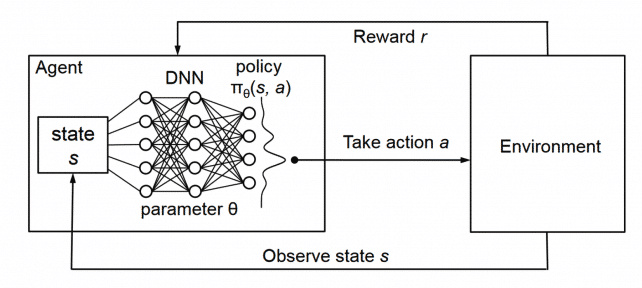
\includegraphics[width=.80\linewidth]{figures/qsys}
    \caption{DQN RL Architecture \cite{qsys}}
    \label{fig:q}
\end{figure}
For the RLPlayer, the agent, to make a decision on what action to take, the game state will be passed through the feedforward trained deep Q network upon every single change of state (after each player's turn and on the flop, turn, river - see \cite{gloss} for poker terminology). Of course, the DQN will be trained through self play, until an optimal poker bot AI converges. Appendix \ref{dqnmodel} displays the few lines of code written in Keras (another python ML library, similar to PyTorch) to build a basic 5 layer neural network.

\section{Python Poker Environment}
Along with research, time has been put into the setup and testing of the chosen poker environment, to ensure feasibility of a properly functioning poker playing game. Once this is tested, time can be spent investigating PyTorch and it's integration to the poker bot and it's environment for training through self play.
\subsection{PyPokerEngine}
After exploring many options online, a well developed poker game engine written in Python has been chosen to utilize for the environment. The library can be found on GitHub \cite{pokergit} as well as supporting documentation for reinforcement learning users \cite{pokerdoc}, another reason it was chosen for this project. You can play against your AI via a console, through a GUI, or run a simulation of any number of rounds of AI vs AI, or a combination of bots. The library comes with built in bots, such as a fish player, fold player, random and honest players, which will be used for the training of our reinforcement learning (RL) bot. Appendix \ref{ppe} displays just how simple it is to setup an RL bot \cite{pokergit}, where the \textit{declare\_actions} function is where the bot will make decisions on which actions to take based off the feedforward results of the trained neural network.

\subsection{PyPokerGUI}
Playing poker against a tuned AI bot through a console is a tedious and unrealistic task. After spending hours training an AI to play poker, one should be able to test it in an environment that resembles that of a real casino, hence the implementation of GUI (guided user interface) support for the \textit{PyPokerEngine}, called the \textit{PyPokerGUI} \cite{pokergui}. All settings exist in a \textbf{.yaml} file to configure and setup a localhost server to run the python module in any browser. Invoking the following command through a terminal can start the server and initiate the game engine GUI:\\\\
\textbf{python3 -m pypokergui serve poker\_conf.yaml --port 8000 --speed moderate}\\\\
The following figure displays a basic two player game of poker in a browser window:
\begin{figure}[H]
    \centering
    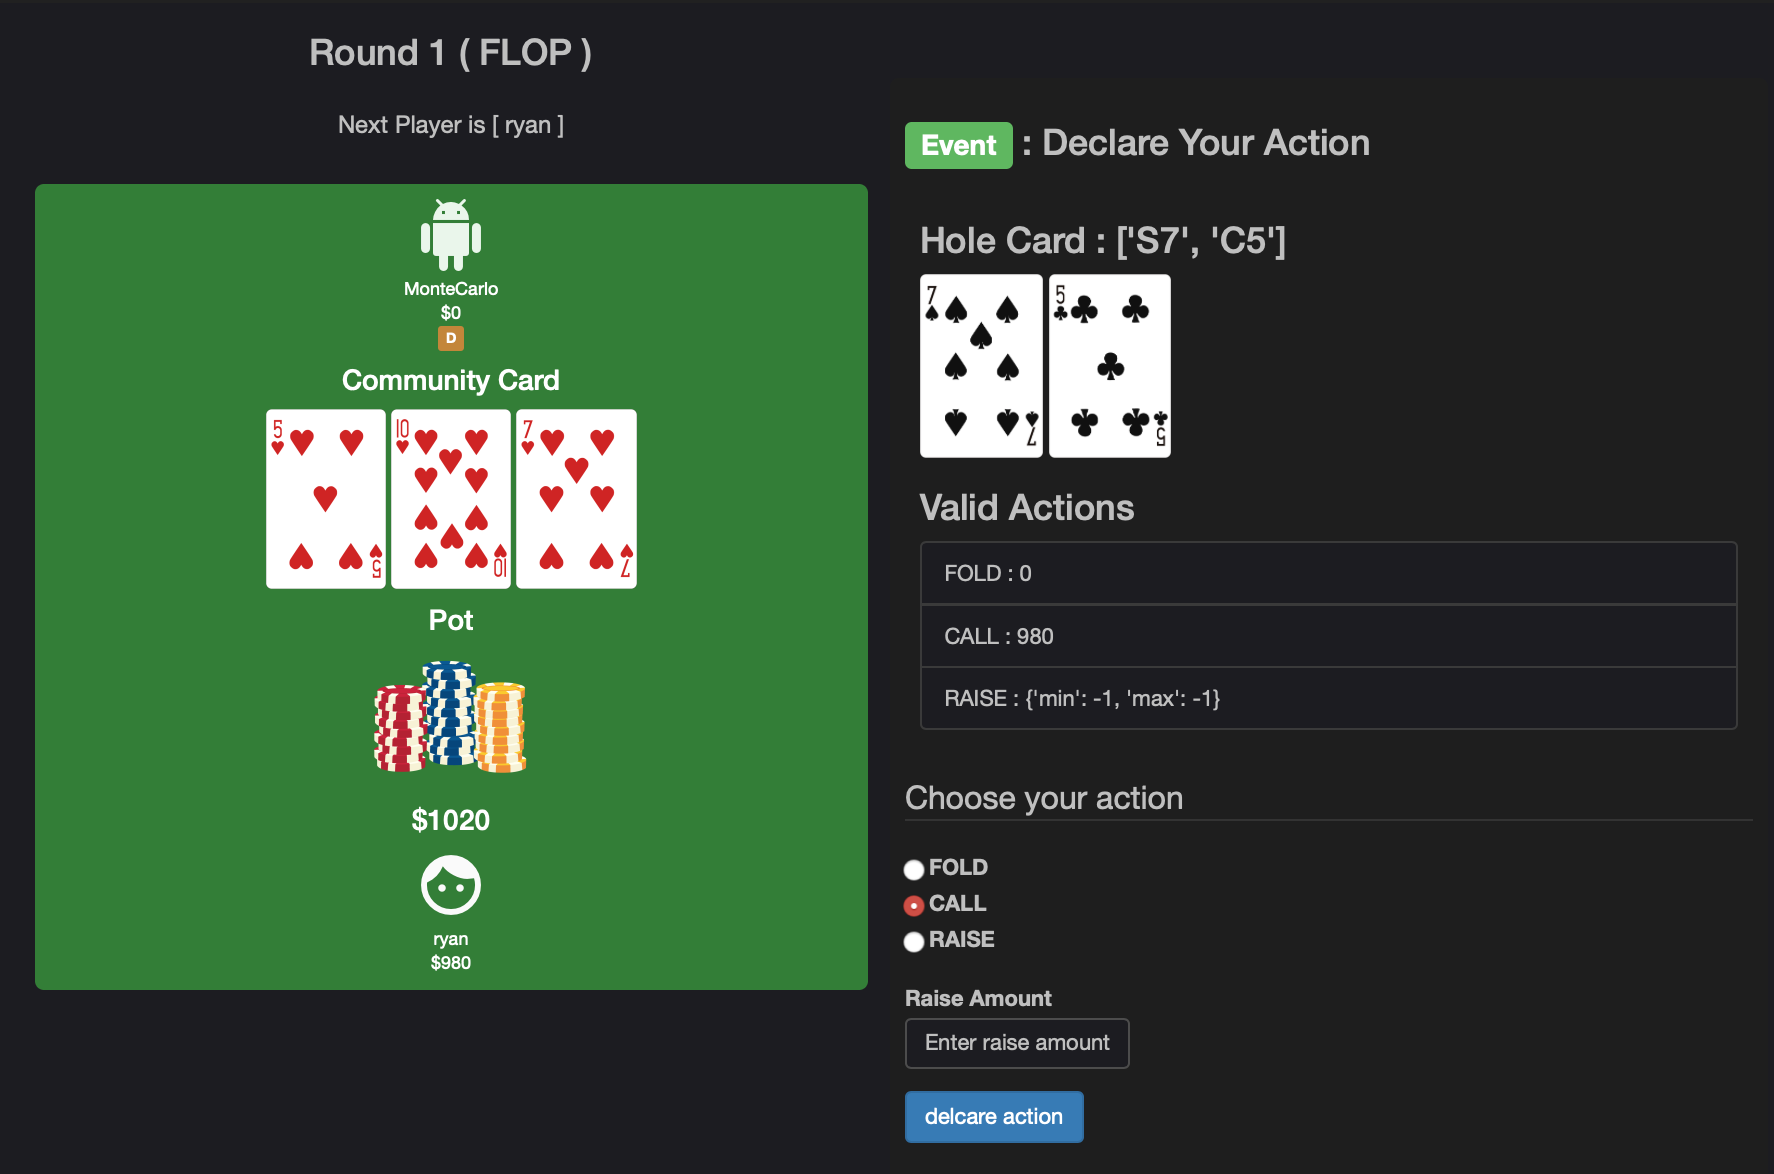
\includegraphics[width=.80\linewidth]{figures/gui}
    \caption{PyPokerGUI Example}
    \label{fig:gui}
\end{figure}
Of course, the game settings can be modified in the \textbf{.yaml} file to play multiple players of different types, different blind sizes, and more. This ultimately provides an excellent testing method for our trained neural network.
\subsection{Training and Simulation}
In order to train the neural network, another method of testing or simulation must be readily available to run at high speeds that does not require user input. Hence, just a few lines can be written in a Python script to begin a simulation of any number of games of poker, while consistently displaying the results.
\begin{minted}[
frame=lines,
framesep=2mm,
baselinestretch=1.2,
fontsize=\scriptsize,
linenos
]{python}
from pypokerengine.api.game import setup_config, start_poker
config = setup_config(max_round=10, initial_stack=100, small_blind_amount=5)
config.register_player(name="p1", algorithm=FishPlayer())
config.register_player(name="p2", algorithm=HonestPlayer())
config.register_player(name="p3", algorithm=RLPlayer())
game_result = start_poker(config, verbose=1)
\end{minted}
Some example results can be seen below:
\begin{minted}[
frame=lines,
framesep=2mm,
baselinestretch=1.2,
fontsize=\scriptsize,
linenos
]{python}
Started the round 10
Street "preflop" started. (community card = [])
"p1" declared "call:10"
"p2" declared "call:10"
"p3" declared "call:10"
Street "flop" started. (community card = ['H7', 'C7', 'C9'])
"p2" declared "call:0"
"p3" declared "call:0"
"p1" declared "call:0"
Street "turn" started. (community card = ['H7', 'C7', 'C9', 'H6'])
"p2" declared "call:0"
"p3" declared "call:0"
"p1" declared "call:0"
Street "river" started. (community card = ['H7', 'C7', 'C9', 'H6', 'HK'])
"p2" declared "call:0"
"p3" declared "call:0"
"p1" declared "call:0"
"['p2']" won the round 10 (stack = {'p1': 90, 'p2': 150, 'p3': 60})
\end{minted}
This simulation will be the core of training the RLPlayer - the neural network. Upon every single action (represented by each new line in the code above) , the player will backpropogate through it's network to tune the gains and minimize the error function, until a best fit is reached.

\section{PyTorch Reinforcement Learning}
There are many libraries that implement the many various concepts and architectures of machine learning in Python, such as TensorFlow, Theano, PyTorch, and more. PyTorch has been chosen as it is the most user friendly, while it still preserves high speeds as it's core is written in C++. It will be integrated with the PyPokerEngine environment to train, test and play the RL bot. Techniques to develop numerous types of RL agents will be employed, including Deep Q Neural Networks and Neural Fictitious Self-Play.

\subsection{RLCard - An RL Toolkit}
RLCard: A Toolkit for Reinforcement Learning in Card Games \cite{rlcard}. This library includes many pre-built agents using TensorFlow instead of PyTorch, and thus provides an excellent, in depth understanding of reinforcement learning and card games. Additionally, there are numerous functioning environments for different types of card games, such as Blackjack, UNO, Rummy, Texas Hold'em and more. Since RLCard possesses the required development for this directed study, it will merely be used as a reference, and benchmark. Further, it's environment will not be utilized for training, as they are less developed and don't contain a GUI. Hence, the required learning to build a successful RL bot will most definitely be gained.
\subsubsection{TensorFlow Training - NFSP Agent}
To assess the computational expense of training a basic NFSP agent in No Limit Hold'em via TensorFlow on a 2015 Mac OS X, a training session was run. Over the span of approximately 45 minutes, the following results were obtained, shown in figure \ref{fig:nfsptf} below.
\begin{figure}[H]
    \centering
    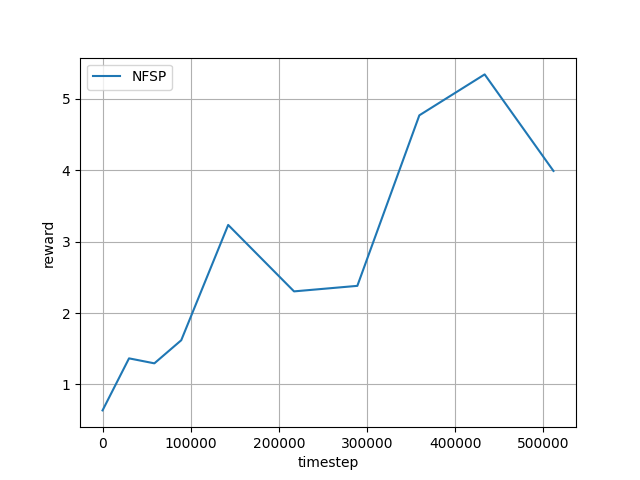
\includegraphics[width=.50\linewidth]{figures/tftrain.png}
    \caption{NFSP Agent Training via TensorFlow in No Limit Hold'em}
    \label{fig:nfsptf}
\end{figure}
Although clearly there is learning taking place, generally, a training agent undergoes plenty more iterations, such as those seen in the following figure.
\begin{figure}[H]
    \centering
    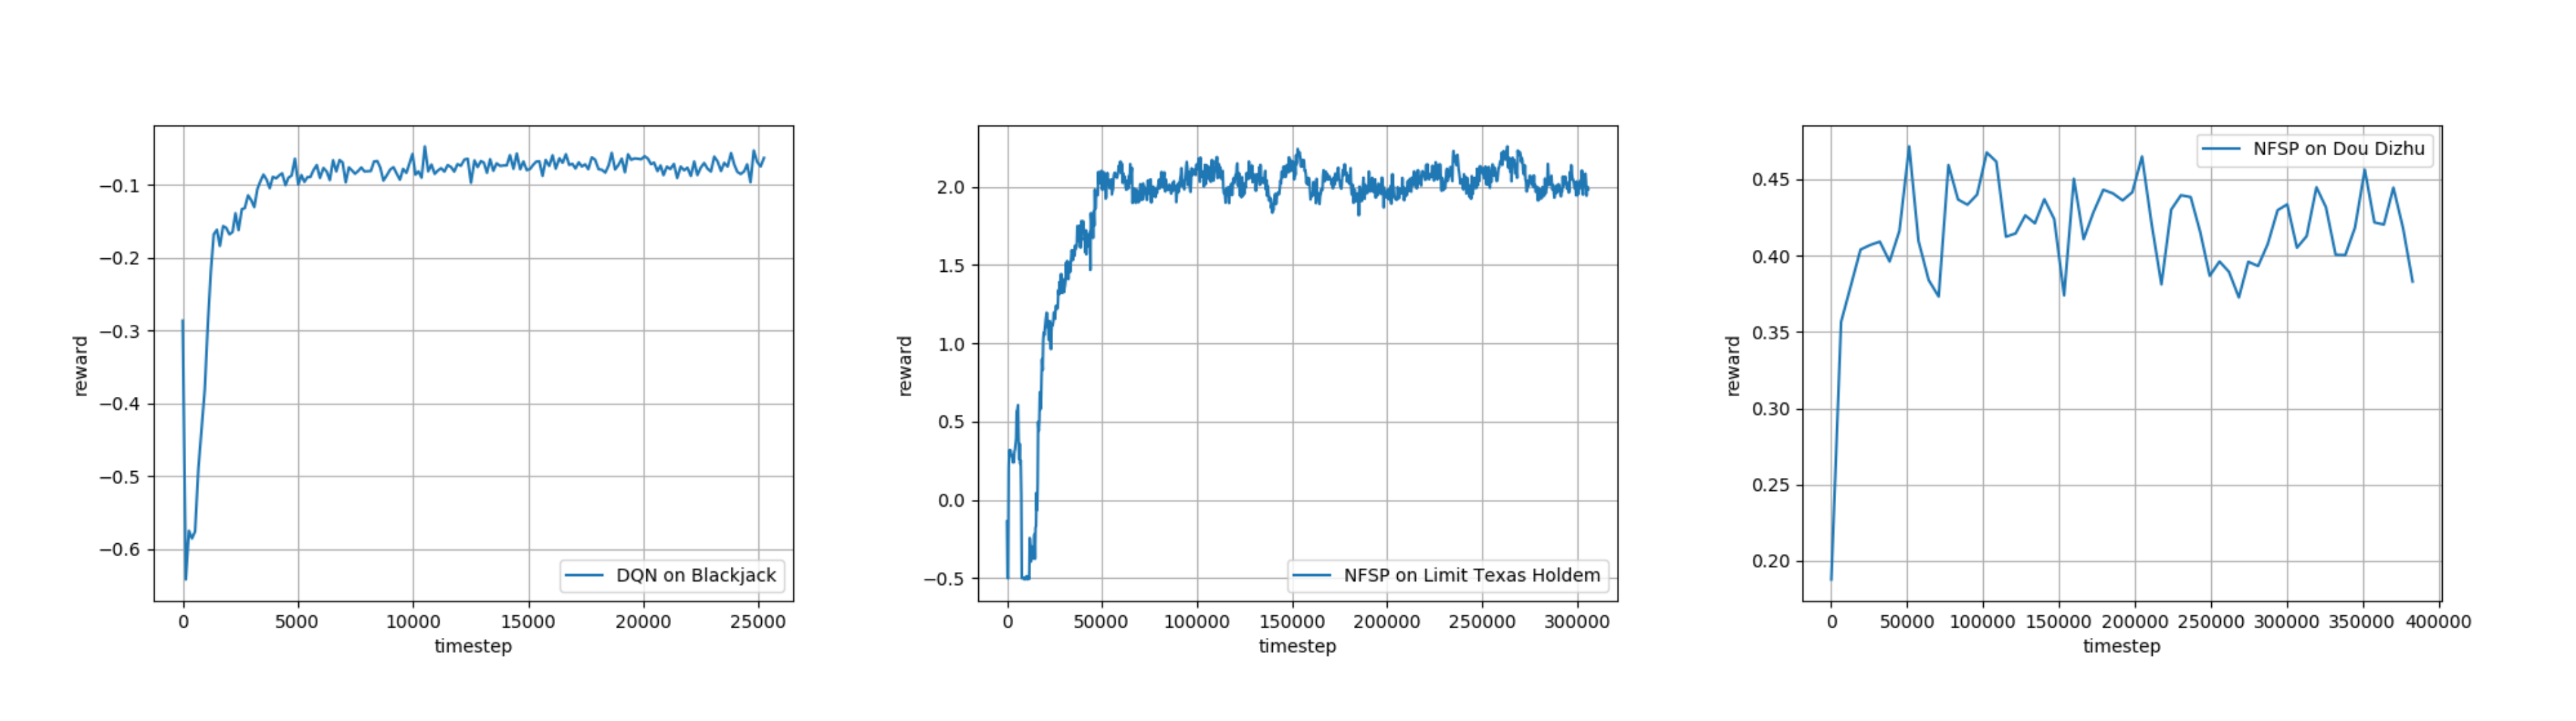
\includegraphics[width=.90\linewidth]{figures/curves.png}
    \caption{RLCard Typical Training Curves \cite{rlcard}}
    \label{fig:rlcurve}
\end{figure}
Thus, it makes much more sense to train the agents on a more expensive piece of hardware, a graphics processing unit - GPU. Since these are built to handle array mathematics in an incredibly short amount of time with respect to a CPU, they can easily shorten the time required to train a neural network. Additionally, Google Colab will be utilized for cloud computing and thus faster training.
\subsection{PyTorch}
Ultimately, the goal is to develop an RL agent through PyTorch, in the PyPokerEngine environment. RLCard serves as a great reference and benchmark to do so.
\subsubsection{DQN and NFSP via PyTorch with PyPokerEngine}
Generally, the RLPlayer should look something like this, depending on the type of agent being implemented. The following Python-pseudo code displays the approximate setup of RLPlayer:

\begin{minted}[
frame=lines,
framesep=2mm,
baselinestretch=1.2,
fontsize=\scriptsize,
linenos
]{python}
from pypokerengine.api.game import setup_config as env
class RLPlayer(BasePokerPlayer):
    def __init__(self):
        # Define init functions for player
        super().__init__()
        self.wins = 0
        self.losses = 0
        # Setup agent
        self.agent = NFSPAgent(scope='nfsp',
                      action_num=env.action_num,
                      state_shape=env.state_shape,
                      hidden_layers_sizes=[128,128],
                      q_mlp_layers=[128,128])
		# Load pre-trained model
		checkpoint_path = 'models/nfsp.pth'
		checkpoint = torch.load(checkpoint_path)
		self.agent.load(checkpoint)

    def declare_action(self, valid_actions, hole_card, round_state):
        # Define action and amount
        # as the output of a feedforward pass through trained NN
        return action, amount

    def receive_game_start_message(self, game_info):
    	# Define state update functions. For example this function:
        self.n_players = env.game_info['player_num']

\end{minted}
The section \textit{declare\_ action} is where the neural net (NN) will operate. It's actions will be determined based off a feedforward pass through it's NN. The sections below will update the states of the RLPlayer based off the game environment. Finally, a \textit{train} function will be setup to train the RLPlayer, through self-play. 
\subsubsection{Google Colab}
Google Colaboratory (Colab) allows anyone to deploy Python projects on remote servers with powerful GPU's \cite{colab}. By merely inputting a link to a Github repository, one can execute computationally expensive programs even though they do not have direct access to hardware, through Colab. It begins with a free trial and then has a fee that is pay per use. This will be explored after a few tests of training the RLPlayer on a basic Mac OS CPU to better understand just how expensive training really is.
\subsection{Agent-Environment Integration}
The PyTorch agent (DQN and NFSP) integration and training with the PyPokerEngine environment is the remaining development for the project. To summarize as a list of the goals for the oncoming 4 weeks;
\begin{enumerate}
	\item State encoding of available cards, stack size, pot size, call cost, etc.
	\item Reward signal setup, testing and variation (DQN)
	\item Build RLPlayer bot, load trained model for feedforward agent decision making (during play)
	\item Effective, observable learning while training
	\item Testing via Human vs. Bot GUI play
\end{enumerate}

\section{Other Information}
\subsection{Timeline}
A revised timeline for the project can be seen below.\\
\begin{chronology}[3]{1}{15}{\textwidth}
\event{1}{Project Kick-off}
\event[1]{3}{Research}
\event[2]{4}{Environment Development}
\event{4}{Basic Environment and Bots Implemented}
\event{6}{Console Based UI Gameplay for Testing}
\event[4]{6}{RL Dev. and Training}
\event[6]{11}{RL PyTorch Integration to PyPokerEngine}
\event{7}{RLCard Testing and Research}
\event{10}{More Advanced RL AI Bot}
\event[10]{14}{Testing, Training, Competitive Play}
\event{14}{Project Completion}
\event[14]{15}{Documentation}

\end{chronology}
\textbf{Project Timeline for the Summer 2020 Semester, by Week}\\

\subsection{Meeting Schedule}
Meetings will be held at 11am PT, recurring weekly on Tuesdays.

% ADD BIBLIOGRAPHY
\newpage
\begin{flushleft}
\nocite{*}
\bibliographystyle{IEEE/IEEEtran}
\bibliography{IEEE/IEEEabrv,IEEE/biblio}
\end{flushleft}

%APPENDICES
\bigskip
\Large{\textbf{Appendices}}
\appendix
\section{Heads Up Push-or-Fold DQN Model}
\label{dqnmodel}
\normalsize
A basic 5 layer neural network written using Keras in Python.
\begin{minted}[
frame=lines,
framesep=2mm,
baselinestretch=1.2,
fontsize=\scriptsize,
linenos
]{python}
def preflop_model():

    input_n = Input(shape=(16,), name="input")

    x = Dense(32, activation='relu')(input_n)
    x = Dense(64, activation='relu')(x)
    x = Dense(16, activation='relu')(x)
    out = Dense(2)(x)
    model = Model(inputs=[input_n], outputs=out)
    model.compile(optimizer='adam', loss='mse')

    return model
\end{minted}

\section{Basic PyTorch NN}
\begin{minted}[
frame=lines,
framesep=2mm,
baselinestretch=1.2,
fontsize=\scriptsize,
linenos
]{python}
from torch import nn
class Network(nn.Module):
    def __init__(self):
        super().__init__()
        
        # Inputs to hidden layer linear transformation
        self.hidden = nn.Linear(784, 256)
        # Output layer, 10 units - one for each digit
        self.output = nn.Linear(256, 10)
        
        # Define sigmoid activation and softmax output 
        self.sigmoid = nn.Sigmoid()
        self.softmax = nn.Softmax(dim=1)
        
    def forward(self, x):
        # Pass the input tensor through each of our operations
        x = self.hidden(x)
        x = self.sigmoid(x)
        x = self.output(x)
        x = self.softmax(x)
        
        return x
\end{minted}

\section{Basic PyTorch DQN}
\label{dqnNN}
\begin{minted}[
frame=lines,
framesep=2mm,
baselinestretch=1.2,
fontsize=\scriptsize,
linenos
]{python}
class DQN(nn.Module):

    def __init__(self, h, w, outputs):
        super(DQN, self).__init__()
        self.conv1 = nn.Conv2d(3, 16, kernel_size=5, stride=2)
        self.bn1 = nn.BatchNorm2d(16)
        self.conv2 = nn.Conv2d(16, 32, kernel_size=5, stride=2)
        self.bn2 = nn.BatchNorm2d(32)
        self.conv3 = nn.Conv2d(32, 32, kernel_size=5, stride=2)
        self.bn3 = nn.BatchNorm2d(32)

        # Number of Linear input connections depends on output of conv2d layers
        # and therefore the input image size, so compute it.
        def conv2d_size_out(size, kernel_size = 5, stride = 2):
            return (size - (kernel_size - 1) - 1) // stride  + 1
        convw = conv2d_size_out(conv2d_size_out(conv2d_size_out(w)))
        convh = conv2d_size_out(conv2d_size_out(conv2d_size_out(h)))
        linear_input_size = convw * convh * 32
        self.head = nn.Linear(linear_input_size, outputs)

    # Called with either one element to determine next action, or a batch
    # during optimization. Returns tensor([[left0exp,right0exp]...]).
    def forward(self, x):
        x = F.relu(self.bn1(self.conv1(x)))
        x = F.relu(self.bn2(self.conv2(x)))
        x = F.relu(self.bn3(self.conv3(x)))
        return self.head(x.view(x.size(0), -1))
\end{minted}
\section{PyPokerEngine Player Setup}
\label{ppe}
\begin{minted}[
frame=lines,
framesep=2mm,
baselinestretch=1.2,
fontsize=\scriptsize,
linenos
]{python}
from pypokerengine.players import BasePokerPlayer
from pypokerengine.api.emulator import Emulator
from pypokerengine.utils.game_state_utils import restore_game_state

from mymodule.poker_ai.player_model import SomePlayerModel

class RLPLayer(BasePokerPlayer):

    # Setup Emulator object by registering game information
    def receive_game_start_message(self, game_info):
        player_num = game_info["player_num"]
        max_round = game_info["rule"]["max_round"]
        small_blind_amount = game_info["rule"]["small_blind_amount"]
        ante_amount = game_info["rule"]["ante"]
        blind_structure = game_info["rule"]["blind_structure"]
        
        self.emulator = Emulator()
        self.emulator.set_game_rule(player_num, max_round, small_blind_amount, ante_amount)
        self.emulator.set_blind_structure(blind_structure)
        
        # Register algorithm of each player which used in the simulation.
        for player_info in game_info["seats"]["players"]:
            self.emulator.register_player(player_info["uuid"], SomePlayerModel())

    def declare_action(self, valid_actions, hole_card, round_state):
        game_state = restore_game_state(round_state)
        # decide action by using some simulation result
        # updated_state, events = self.emulator.apply_action(game_state, "fold")
        # updated_state, events = self.emulator.run_until_round_finish(game_state)
        # updated_state, events = self.emulator.run_until_game_finish(game_state)
        if self.is_good_simulation_result(updated_state):
            return # you would declare CALL or RAISE action
        else:
            return "fold", 0
\end{minted}


\end{document}
